\chapter{数据模型}

数据本身只反映出现象,因此我们的目的不仅仅是搜集数据本身,而是通过数据发现背后的机理和规律——
不只是回答“怎么样”,更重要的是回答“为什么”。而发现数据中规律的重要方法就是数据模型。

\section{交通流模型}

以一条道路上的交通状态为例,我们可以用流量$q$、密度$k$、速度$v$三个指标来描述。
其中根据物理守恒定律很容易推导出$q=k\cdot v$,另一方面密度$k$和速度$v$之间的关系就不是那么直观了。对于这种未知的关系,我们可以用一个函数$v=f(k)$表示,$f$的数学定义就代表了速度和密度之间的关系,也是路段上交通状态变化的背后机理。

为了找出合适的函数$f$我们要从实际出发,首先通过各种手段实际观测道路上的流量、密度、速度。
直接从现实世界观测到的数据称为\emph{实测数据(empirical data)}%
\sidenote{empirical是一个哲学词汇,反义词是ideological。分别表示基于现实世界的的和基于意识形态的证据}
,大量数据如果以数字表格形式存在,我们很难理解。
因此第一步一般是将数据可视化,绘制成某种图形。

路段流密速数据一般可视化方法是以将每一条记录画作一个数据点,横坐标表示密度、纵坐标表示速度或流量。实测数据绘制后一般呈现出类似\cref{fig:empirical-qkv}的形态,从中马上可以看出一些规律。
例如从左图中速度和密度之间的关系,可以看出随着密度增加速度总体呈下降趋势;而且密度较小时速度下降不明显。从右图中流量和密度之间的关系,可以看出随着密度增加流量呈先上升后下降的趋势。

\begin{figure*}
    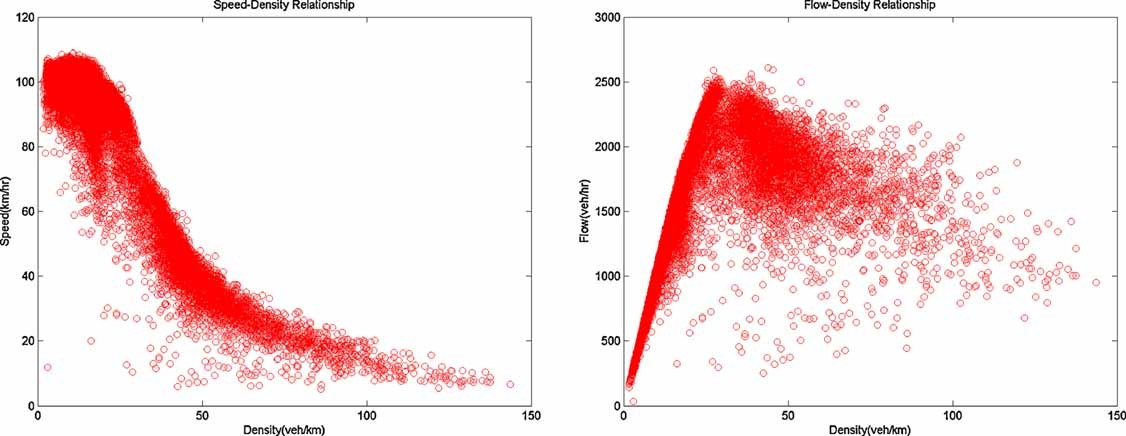
\includegraphics[width=\linewidth]{images/empirical-qkv.jpg}
    \caption{路段流量、密度、速度的典型实测数据}
    \label{fig:empirical-qkv}
\end{figure*}

由于我们已经知道$q=k\cdot v$,也就是说知道$k$,$v$就能计算出$q$,因此流量$q$对于我们来说是\emph{冗余数据(redundant data)},在后续分析中可以舍弃\sidenote{冗余数据并非没有价值,可以用于验证数据有效性。这里直接舍弃是为了简化讨论。}。此时我们面临的问题是,定义一个函数
\begin{equation}
    v=f(k)
\end{equation}
让该函数的图像与实测数据尽量符合,在数学上称为\emph{拟合问题}。

为了确定函数$f$的定义我们需要回答两个问题。第一个问题是函数的基本形态是什么?例如是直线、抛物线、还是指数曲线。这里我们假设$f$的图像是一条直线\sidenote{合理选取函数形式要综合考虑很多因素,没有标准答案,需要结合经验和对数据本身的理解。}
,也可以说$f$是\emph{线性函数}。
对于线性函数我们可以写出公式
\begin{equation}\label{eq:linear-kv}
    v = a\cdot k + b
\end{equation}
其中$a$和$b$是未知\emph{参数(parameter)}。
解析几何告诉我们$a$,$b$参数取值决定直线的形态,因此第二个个问题是$a$、$b$取值多少函数$f$与实测数据吻合\emph{最好}。

\section{线性回归}
为了确定\cref{eq:linear-kv}中的参数$a$、$b$我们需要用到一种叫做\emph{线性回归}的数学方法。
不过在正式介绍线性回归前,我们可以看一个简化的例子,方便理解为什么需要线性回归。

假设我们实测的数据只有两组,即两个不同时刻的密度和速度,分别写作$[p_1=(k_1, v_1), p_2=(k_2, v_2)]$,其中$p$代表数据点(point)。
此时图上只有两个数据点,函数$f$的图像是一条直线,显然当它同时穿过$p_1$、$p_2$时对数据的拟合最好。如何确定此时$a$、$b$的取值?

我们可以通过线性方程组来求解$a$、$b$。由于直线穿过两个数据点,以下两个方程必定成立:
\begin{align*}
    v_1 = a\cdot k_1 + b \\
    v_2 = a\cdot k_2 + b
\end{align*}
其中$a$、$b$是需要求解的未知数,可以用高斯消元法求解。
但这里我们先不求解,而是先把方程组写成线性代数的矩阵形式,方便后面的讨论。
\begin{equation}
    \begin{bmatrix}
        v_1\\
        v_2
    \end{bmatrix}=
    \begin{bmatrix}
        k_1 & 1\\
        k_2 & 1
    \end{bmatrix}\cdot
    \begin{bmatrix}
        a\\
        b
    \end{bmatrix}
\end{equation}